\documentclass[9pt,twocolumn,twoside,]{pnas-new}

% Use the lineno option to display guide line numbers if required.
% Note that the use of elements such as single-column equations
% may affect the guide line number alignment.


\usepackage[T1]{fontenc}
\usepackage[utf8]{inputenc}

% tightlist command for lists without linebreak
\providecommand{\tightlist}{%
  \setlength{\itemsep}{0pt}\setlength{\parskip}{0pt}}


% Pandoc citation processing
\newlength{\cslhangindent}
\setlength{\cslhangindent}{1.5em}
\newlength{\csllabelwidth}
\setlength{\csllabelwidth}{3em}
\newlength{\cslentryspacingunit} % times entry-spacing
\setlength{\cslentryspacingunit}{\parskip}
% for Pandoc 2.8 to 2.10.1
\newenvironment{cslreferences}%
  {}%
  {\par}
% For Pandoc 2.11+
\newenvironment{CSLReferences}[2] % #1 hanging-ident, #2 entry spacing
 {% don't indent paragraphs
  \setlength{\parindent}{0pt}
  % turn on hanging indent if param 1 is 1
  \ifodd #1
  \let\oldpar\par
  \def\par{\hangindent=\cslhangindent\oldpar}
  \fi
  % set entry spacing
  \setlength{\parskip}{#2\cslentryspacingunit}
 }%
 {}
\usepackage{calc}
\newcommand{\CSLBlock}[1]{#1\hfill\break}
\newcommand{\CSLLeftMargin}[1]{\parbox[t]{\csllabelwidth}{#1}}
\newcommand{\CSLRightInline}[1]{\parbox[t]{\linewidth - \csllabelwidth}{#1}\break}
\newcommand{\CSLIndent}[1]{\hspace{\cslhangindent}#1}


\templatetype{pnasresearcharticle}  % Choose template

\title{Diversité des collaborations des élèves du cours BIO500 à l'hiver
2022}

\author[a]{Marguerite Duchesne}
\author[a]{Florian Jordan}
\author[a]{Anthony St-Pierre}
\author[a]{Simon Grégoire}
\author[a]{Francis Lessard}

  \affil[a]{Université de Sherbrooke, Départment de biologie, 2500
Boulevard de l'Université, Sherbrooke, Québec, J1K 2R1}


% Please give the surname of the lead author for the running footer
\leadauthor{}

% Please add here a significance statement to explain the relevance of your work
\significancestatement{}


\authorcontributions{}



\correspondingauthor{\textsuperscript{} }

% Keywords are not mandatory, but authors are strongly encouraged to provide them. If provided, please include two to five keywords, separated by the pipe symbol, e.g:
 \keywords{  Collaborations |  Réseau écologique |  Travaux d'équipe  } 

\begin{abstract}
Nous nous sommes intéréssés aux collaborations des élèves de
l'Université de Sherbrooke à l'hiver 2022 lors de travaux d'équipe
pendant leur parcours dans le baccalauréat en biologie. Pour ce faire,
nous avons dressé un réseau entre tous les étudiants qui ont suivi le
cours de méthodes en écologie computationnelle (BIO500) lors de la
session d'hiver 2022 et leurs collaborateurs au long de leur parcours
universitaire. Nous avons comparé le nombre total de collaborations de
chaque étudiant ainsi que le nombre de collaborations différentes de
chaque étudiant dans le but de déterminer s'ils ont tendance à conserver
les mêmes équipes ou non. Nous avons aussi observé l'impact que le cours
de méthodes analytiques en biologie (TSB303) possédait sur le réseau
puisque ce dernier comporte un travail d'équipe comprenant jusqu'à 9
personnes. Nous avions un soupçon qu'un travail de cette ampleur
modifierait beaucoup le réseau final. On a facilement pu identifier sur
le réseau les groupes de travail qui se sont maintenus à travers le
baccalauréat, ce qui prouve que les étudiants n'avaient pas tendance à
diversifier leurs collaborations.
\end{abstract}

\dates{This manuscript was compiled on \today}
\doi{\url{www.pnas.org/cgi/doi/10.1073/pnas.XXXXXXXXXX}}

\begin{document}

% Optional adjustment to line up main text (after abstract) of first page with line numbers, when using both lineno and twocolumn options.
% You should only change this length when you've finalised the article contents.
\verticaladjustment{-2pt}



\maketitle
\thispagestyle{firststyle}
\ifthenelse{\boolean{shortarticle}}{\ifthenelse{\boolean{singlecolumn}}{\abscontentformatted}{\abscontent}}{}

% If your first paragraph (i.e. with the \dropcap) contains a list environment (quote, quotation, theorem, definition, enumerate, itemize...), the line after the list may have some extra indentation. If this is the case, add \parshape=0 to the end of the list environment.

\acknow{}

\hypertarget{introduction}{%
\section{Introduction}\label{introduction}}

On entend souvent l'expression « Ah que le monde est petit ! » lorsque
deux personnes se retrouvent à avoir une connexion qu'on ne suspectait
pas. Certaines études se sont intéressées à ce principe selon lequel
tout le monde est lié à un certain niveau. Milgram (1967) s'est penché
sur le sujet et a testé cette hypothèse selon laquelle deux personnes
pigées au hasard devraient avoir un lien rapproché entre eux (1). Ce
principe peut également s'appliquer à l'écologie. Du point de vue de
l'évolution, toutes les espèces sont reliées par un ancêtre commun (2).
Les réseaux trophiques présentent aussi ce genre de dynamique (2). Ce
modèle de « petit monde » peut donc s'appliquer à grande et petite
échelle. Nous avons voulu observer cette théorie à très petite échelle
dans le baccalauréat de la 59e cohorte d'écologie de l'Université de
Sherbrooke. L'école forme les futurs travailleurs de demain, et avoir un
grand nombre de collaborations à l'université peut être bénéfique si on
se fie aux recommandations de plusieurs firmes aidant les travailleurs à
optimiser leurs capacités au travail. Un réseau de collaborations
diversifié entraîne un engagement plus élevé des employés, une meilleure
rétention et plus d'innovation (3). Nous nous sommes donc posés la
question si le réseau de collaborations entre les étudiants du
baccalauréat en écologie favorisait la diversité des collaborations.
Plus spécifiquement, nous avons étudié si les élèves ayant un grand
nombre de collaborations ont davantage tendance à diversifier leurs
partenaires. En effet, il est intéressant de voir si les étudiants ont
plusieurs groupes de collaborateurs ou si, au cours du baccalauréat, ils
ont entretenu des liens avec les mêmes personnes. Nous avons également
vérifié si le cours de méthodes analytiques en biologie (TSB303) a eu un
grand effet dans le réseau de collaborations, puisque dans ce cours, le
travail était pour la plupart en équipes de 9. On peut donc s'imaginer
qu'à lui seul, ce cours ajoute beaucoup de collaborations entre les
étudiants. Le réseau de collaborations entre les étudiants ayant plus de
30 collaborations sera aussi produit pour observer si la dynamique des
liens entre étudiants change dans cette situation.

\hypertarget{muxe9thode}{%
\section{Méthode}\label{muxe9thode}}

La classe de BIO500 de la session d'hiver 2022 s'est divisée en 9
équipes. Chaque élève de ces équipes a compilé l'ensemble des cours pour
lesquels des travaux d'équipe ont été réalisés lors de son baccalauréat.
Ces informations ainsi que les données considérées pertinentes reliées à
ces cours ont été compilées dans une première table commune à l'équipe.
Ils ont également compilé dans une seconde table le nom de chaque
coéquipier ainsi que de leurs collaborateurs. Pour chacun des étudiants,
l'année de début de leur baccalauréat, le nom de leur programme et leur
participation au régime coopératif ont été ajoutés. Ils ont terminé la
compilation des données par une troisième table, dans laquelle se trouve
l'ensemble des collaborations, c'est-à-dire leurs liens collaboratifs
avec d'autres étudiants et le travail d'équipe correspondant à ce lien.

Une fois la compilation des données réalisée par chaque équipe, celle-ci
fut partagée et mise en commun. Les équipes avaient alors la tâche de
fusionner l'ensemble des données afin de n'avoir que trois tables
contenant l'ensemble des données de la classe. Ceci a été effectué dans
le logiciel R. Au préalable, chaque équipe a dû standardiser les données
de l'ensemble des équipes afin d'obtenir une conformité au sein des
différentes tables. Ces données ont ensuite été injectées dans le
système de gestion de données SQLite3. Afin de répondre à la question
posée, les données d'intérêt ont été extraites via des requêtes et
ensuite analysées. Les représentations visuelles des réseaux ont été
effectuées grâce au package ``Igraph'' du locigiel R. Finalement, le
package ``targets'' a été utilisé afin d'automatiser l'ensemble du
processus et d'augmenter la reproductibilité de la démarche.

\hypertarget{ruxe9sultats}{%
\section{Résultats}\label{ruxe9sultats}}

Pour mieux illustrer les réponses aux questions, plusieurs figures
présenteront les liens entre les étudiants.

\begin{figure}
\centering
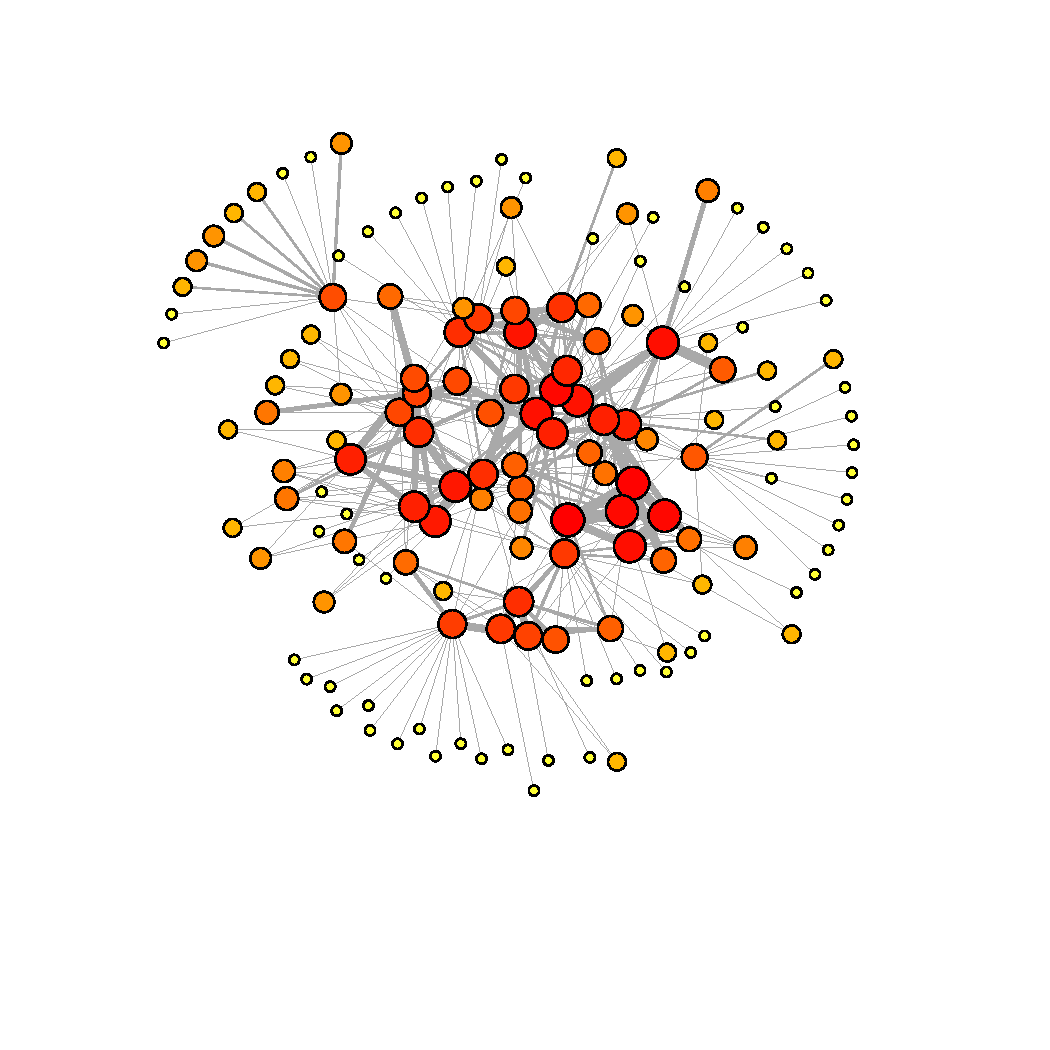
\includegraphics[width=0.5\textwidth,height=0.4\textheight]{"../results/figure1.png"}
\caption{Réseau de collaborations des étudiants du cours BIO500 l'hiver
2022.La grandeur et la couleur des noeuds sont déterminées par une
comparaison relative du nombre de collaborations de chaque élève, les
cercles les plus petits et jaunes correspondent à une seule
collaboration. La largeur des liens correspond au nombre de
collaborations entre la paire d'étudiants. \label{fig:plot1}}
\end{figure}

La figure \ref{fig:plot1} représente le réseau de toutes les
collaborations des étudiants du cours de méthodes en écologie
computationnelle (BIO500) à l'hiver 2022. Dans ce contexte, la moyenne
de liens par étudiant est de 10.67, la distance maximale entre deux
étudiants est de 5 liens et la modularité du réseau est de 0.635.

La figure \ref{fig:plot2} met en évidence les collaborations du cours
TSB303. Les paramètres du réseau se voient changés en l'absence du cours
TSB303. La moyenne du nombre de collaborations par étudiant est de
11.13, la distance maximale entre deux étudiants est de 6 liens alors
que la modularité du réseau est de 0.497.

\begin{figure}
\centering
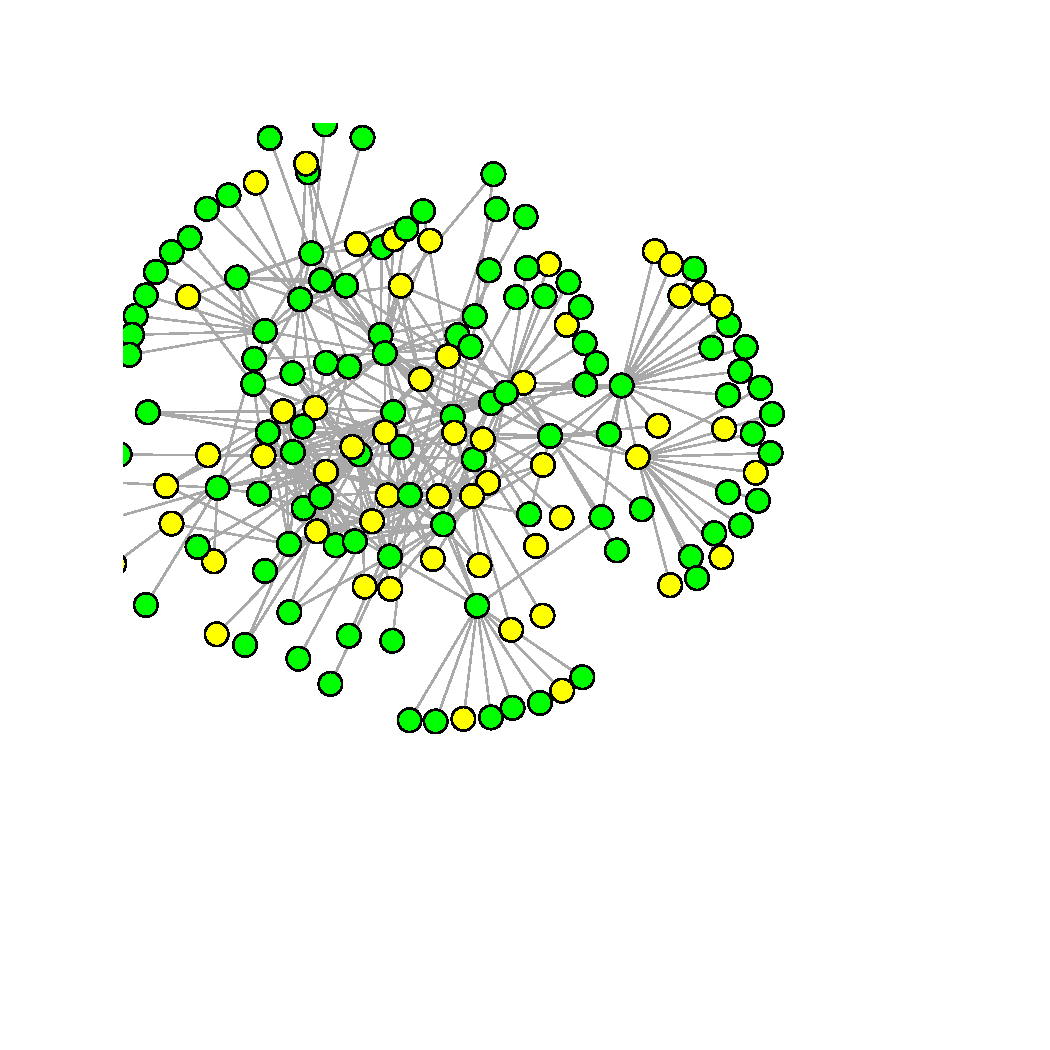
\includegraphics[width=0.5\textwidth,height=0.4\textheight]{"../results/figure2.png"}
\caption{Réseaux de collaborations des élèves du cours BIO500 à l'hiver
2022 avec et sans le cours TSB303. À gauche, on voit le réseau des
différentes collaborations sans celles provenant du cours TSB303 et à
droite, le réseau de toutes les collaborations, mais les liens mis en
gras représentent ceux du cours TSB303. les noeuds jaunes représentent
des élèves n'étant pas en écologie alors que les noeuds verts sont des
étudiants en écologie.\label{fig:plot2}}
\end{figure}

La figure \ref{fig:plot3} est le réseau des différentes collaborations
depuis le début du baccalauréat entre les étudiants du cours de méthodes
en écologie computationnelle (BIO500) à l'hiver 2022 possédant 30
collaborations et plus. Dans cette situation, la modularité du réseau
est de 0.621.

\begin{figure}
\centering
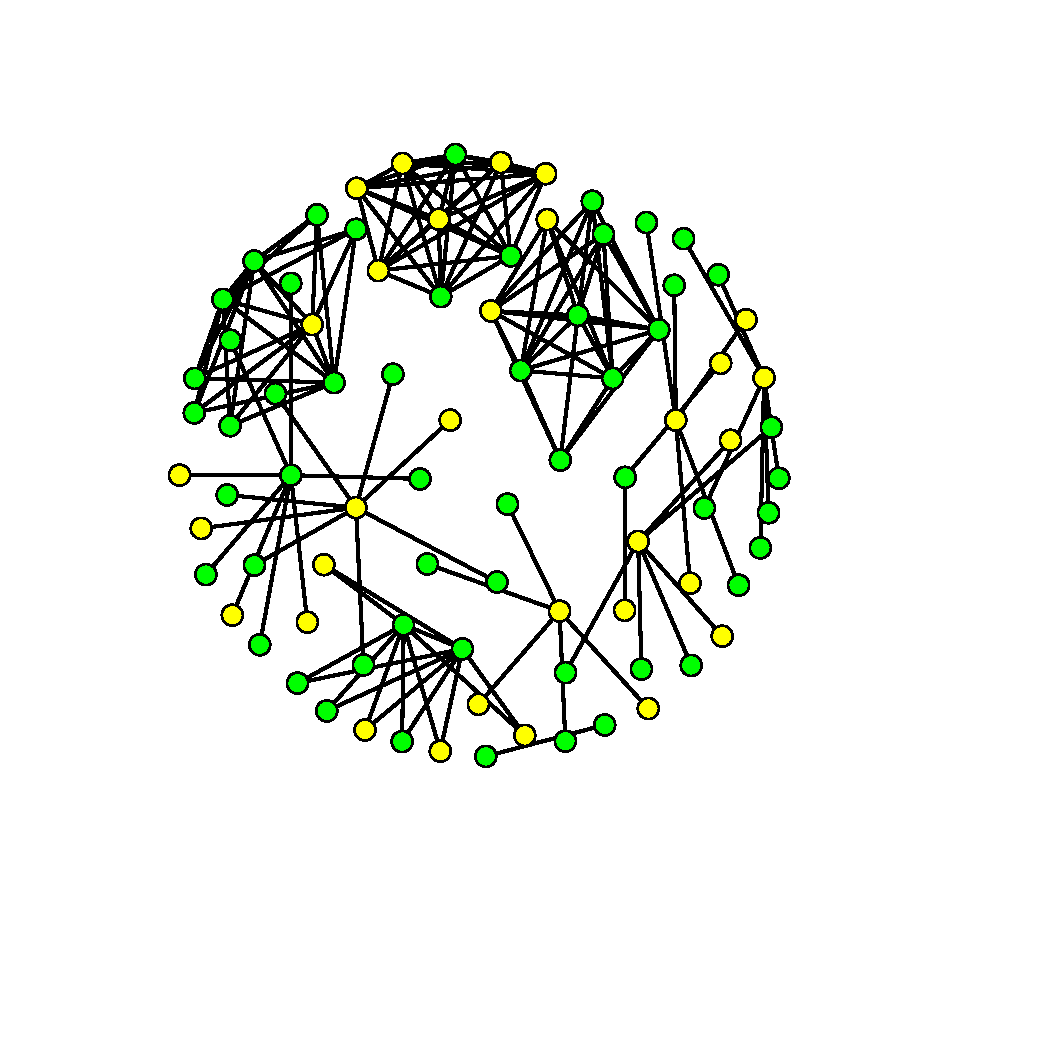
\includegraphics[width=0.5\textwidth,height=0.4\textheight]{"../results/figure3.png"}
\caption{Réseau de collaborations entre les élèves du cours BIO500 à
l'hiver 2022 qui ont plus de 30 collaborations. La grandeur et la
couleur des noeuds sont proportionnelles au nombre de collaborations de
chaque élève. La largeur des liens correspond au nombre de
collaborations entre la paire d'étudiants. \label{fig:plot3}}
\end{figure}

Notre quatrième et dernière figure (\ref{fig:plot4}) représente le
nombre d'étudiants pour différents nombres de collaborations (a) ainsi
que le nombre de collaborations différentes par étudiant (b), c'est à
dire le nombre de personnes distinctes avec qui ils ont coopéré pendant
le baccalauréat en écologie. Ces résultats sont aussi présentés sans le
cours TSB303 (c et d). La moyenne des collaborations différentes entre
étudiants est de 4.88 avec le cours TSB303 et de 4.83 sans le cours
TSB303.

\begin{figure}
\centering
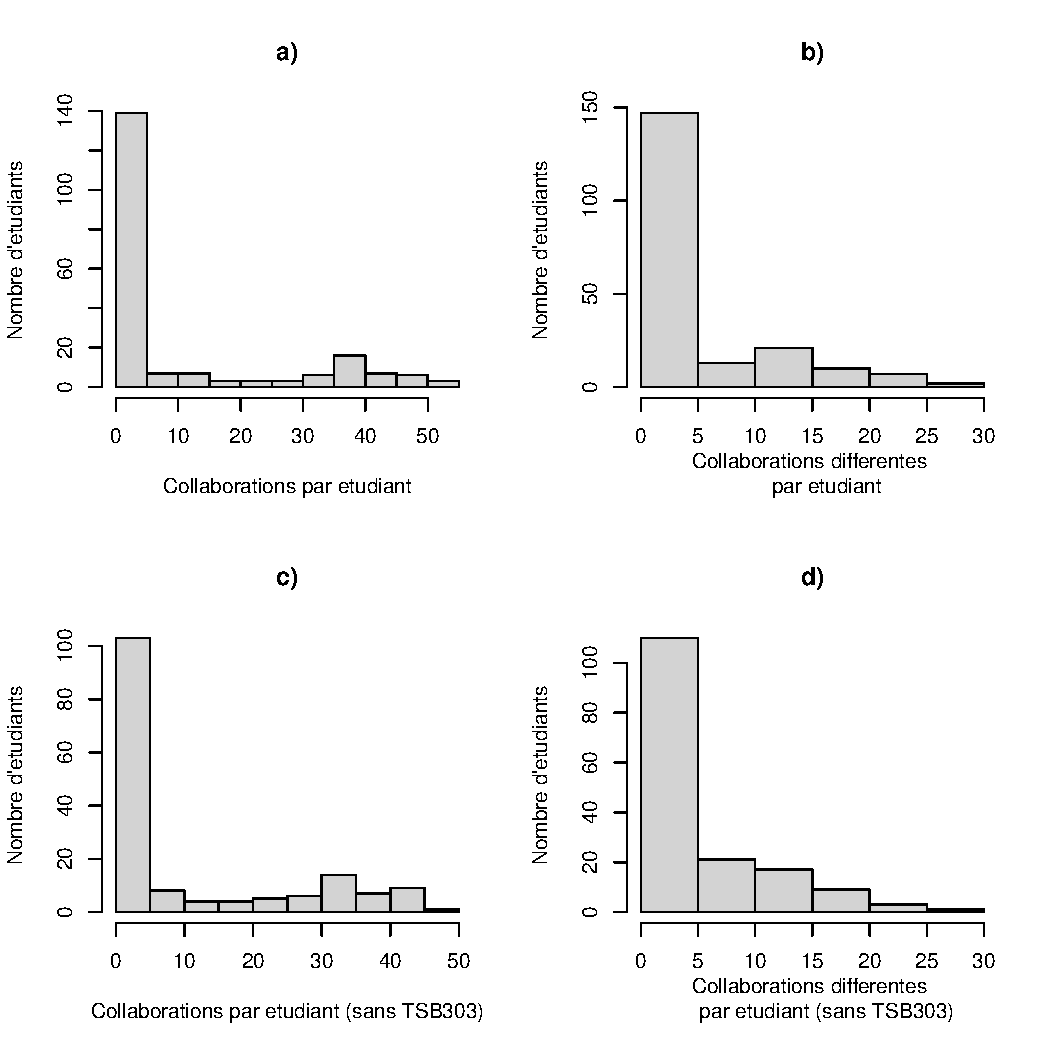
\includegraphics[width=0.5\textwidth,height=0.4\textheight]{"../results/figure4.png"}
\caption{Comparaison des collaborations totales et différentes des
élèves du cours BIO500 à l'hiver 2022 avec et sans le cours TSB303. (a)
Le nombre de collaborations par étudiant. (b) Le nombre de
collaborations différentes par étudiant. (c) Le nombre de collaborations
par étudiant snas TSB303. (d) Le nombre de collaborations différentes
par étudiant sans le cours TSB303. \label{fig:plot4}}
\end{figure}

\hypertarget{discussion}{%
\section{Discussion}\label{discussion}}

Rapidement, il est possible de remarquer que les élèves ont tendance à
conserver les mêmes collaborateurs. En terme d'exemple, les trois
personnes dans le réseau de base ayant plus de 50 collaborations ont
également moins de 15 collaborateurs différents. Les liens larges
permettent de distinguer que plusieurs les paires d'élèves ont de
multiples collaborations ensembles. Cela est également visible par la
forte modularité du réseau de base de 0.635. Cela suggère donc que
plusieurs sous-groupes dans le réseau ont peu de collaboration entre
eux, ce qui limite le nombre de collaborateurs différents. La grande
quantité de petits noeuds jaunes dans la figure \ref{fig:plot1} explique
aussi la faible moyenne de collaborations par étudiant de 10.67.

Jugeant que 30 collaborations et plus correspondaient à un grand nombre
de collaborations, nous avons donc porté notre réflexion sur les raisons
qui avaient mené ces gens à obtenir autant de collaborations. On peut
voir que la modularité du réseau de la figure \ref{fig:plot3} de 0.621
est très similaire à celle du réseau complet. Cela semble signifier que
même en l'absence des individus ayant peu de collaborations, des
sous-groupes de collaborateurs sont visibles dans le réseau. Une méthode
couramment utilisée en écologie est le calcul du coefficient de Jaccard
(4). Cela permettrait de quantifier l'hétérogénéité des interactions par
l'analyse des liens partagés. Il serait donc possible de distinguer des
similarités dans la source du grand nombre de collaborations de ces
étudiants (5).

Lorsqu'on enlève le cours TSB303 aux collaborations, on voit une
augmentation de la moyenne de collaborations par étudiant de 10.67 à
11.13 ainsi qu'un légère diminution du nombre de collaborations par
étudiant de 4.88 à 4.83 (Figure \ref{fig:plot4}. Cela est compréhensible
puisque le travail d'équipe de ce cours est la seule collaboration pour
de nombreux étudiants du réseau. Ce qui est intéressant est que la
modularité diminue grandement de 0.635 avec le cours TSb303 à 0.497 sans
le cours TSB303. Donc, l'ajout des étudiants dont la seule collaboration
est celle de TSB303 augmente la formation de sous-groupes dans le
réseau. Il faut également considérer que certaines personnes n'ont pas
ajouté les collaborations réalisées pour ce cours dans les données
brutes probablement en raison d'un oubli. Il serait fort probable que le
cours TSB303 ait un effet supérieur sur les paramètres du réseau en
réalité. Il est clair que les grandes équipes dans ce cours ont augmenté
le nombre de collaborations différentes chez les élèves. Cependant, le
type de collaboration utilisé pour le cours TSB303 ne semble pas
recommandable. Une grande quantité de collaborateurs ne semble pas
toujours être la solution pour augmenter les bienfaits de la
collaboration. En effet, il faut également mentionner la qualité des
collaborations. Ce type de travail court et ayant beaucoup de
collaborateurs ne laisse pas beaucoup de marge pour que le travail soit
réparti équitablement. La bonne communication entre tous les
collaborateurs devient également un défi. À terme, il semble donc
justifié de ne pas comparer ce type de collaboration aux autres.

\hypertarget{conclusion}{%
\section{Conclusion}\label{conclusion}}

Le réseau de collaborations nous montre que le élèves du cours BIO500 à
l'hiver 2022 ont davantage été portés à conserver les mêmes
collaborateurs tout au long de leur parcours universitaire. Il serait
également possible d'approfondir nos connaissances sur la genèse d'un
grand nombre de collaborations via le calcul du coefficient de Jaccard.
Ce faisant, il serait peut-être possible d'orienter les professeurs sur
des pistes d'amélioration en vue de former de meilleurs futurs
travailleurs et ce, en gardant en tête que la qualité prévaut à la
quantité des liens. Néanmoins, nous pouvons d'ores et déjà recommander
la mise en place d'efforts afin d'accentuer le nombre de collaborations
différentes chez les étudiants. Étant les scientifiques de demain, les
élèves peuvent également et devraient toujours être encouragés à prendre
eux-mêmes la décision d'élargir leur cercle de connexions.

\newpage

\hypertarget{bibliographie}{%
\section*{Bibliographie}\label{bibliographie}}
\addcontentsline{toc}{section}{Bibliographie}

\hypertarget{refs}{}
\begin{CSLReferences}{0}{0}
\leavevmode\hypertarget{ref-milgram1967small}{}%
\CSLLeftMargin{1. }
\CSLRightInline{Milgram S (1967) The small world problem.
\emph{Psychology today} 2(1):60--67.}

\leavevmode\hypertarget{ref-montoya2002small}{}%
\CSLLeftMargin{2. }
\CSLRightInline{Montoya JM, Solé RV (2002) Small {World} {Patterns} in
{Food} {Webs}. \emph{Journal of Theoretical Biology} 214(3):405--412.}

\leavevmode\hypertarget{ref-holtzman2011diversify}{}%
\CSLLeftMargin{3. }
\CSLRightInline{Holtzman Y, Anderberg J (2011) Diversify your teams and
collaborate: Because great minds don't think alike. \emph{Journal of
Management Development}.}

\leavevmode\hypertarget{ref-legendre2012numerical}{}%
\CSLLeftMargin{4. }
\CSLRightInline{Legendre P, Legendre L (2012) Numerical ecology, 3rd
english edition, v. 24.}

\leavevmode\hypertarget{ref-delmas2019analysing}{}%
\CSLLeftMargin{5. }
\CSLRightInline{Delmas E, et al. (2019) Analysing ecological networks of
species interactions. \emph{Biological Reviews} 94(1):16--36.}

\end{CSLReferences}



% Bibliography
% \bibliography{pnas-sample}

\end{document}
